\documentclass[UTF8]{ctexart}
\usepackage[linesnumbered,ruled,vlined,boxed]{algorithm2e}
\usepackage{amsthm}
\usepackage{geometry}
\usepackage{graphicx}
\usepackage{mathtools}
\usepackage{minted}
\usepackage{amsmath}
\usepackage{amsfonts}
\usepackage{xpinyin}
\geometry{a4paper}
\title{\textbf{人工智能课程实验1}}
\author{武自厚 20336014 保密管理}
\date{\today}

\newcommand{\diff}{\mathrm{d}}
\newcommand{\var}[1]{\mathtt{#1}}
\newcommand{\func}[2]{\mathtt{#1(\mathnormal{#2})}}

\begin{document}

    \maketitle

    \section{实验目的}

    熟悉Python语言的语法及特性,并以此为基础实现无向图的最短路径算法(Dijkstra算法).

    \section{算法原理}

    \subsection{策略}
    本算法基于“贪心策略”实现,具体表现为:在一次遍历中只考虑已访问结点和未访问
    结点之间\textbf{最短}的边.
    \subsection{数据结构}
    无向图的存储使用邻接表,结点已访问与否的判断以及最短路径表示使用并查集,
    “贪心策略”的实现使用优先队列.
    \subsection{自然语言描述}
    首先,对任意结点$v$赋予“距离”属性且其值为无穷大,即$\var{dist}[v] = \infty$,
    随后将起点的“距离”赋值为0.再对任意节点$v$赋予“前驱”属性,并其值赋值为结点自身,即$v.\pi = v$

    直到所有结点都加入时,重复以下步骤:遍历无向图的每一条边(权为$w$),如果其中一个端点$u$已经访问
    且另一个端点$v$未访问,且$\var{dist}[u] + w < \var{dist}[v]$则将这条边纳入考虑.
    再将所有已经考虑的边中取出权最小的,将其终点的“距离”用起点的“距离”与边权的和取代(即松弛过程),
    并且将终点设为“已访问”,将终点的“前驱”赋值为起点.

    算法结束之后,目标点的“距离”属性即位最短路径长度,通过迭代访问“前驱”属性可以获得该路径上所有结点的序列.

    \section{伪代码实现}
    \subsection{主算法}
    \begin{algorithm*}
		\SetKwInOut{Input}{输入}
		\SetKwInOut{Output}{输出}
        \SetKwData{Left}{left}
		\caption{Dijkstra算法}
		\Input{带权图\(G = \langle V,E \rangle\),初始结点 \(a\), 终止结点\(b\)}
		\Output{\(G\)中从\(a\)到\(b\)的最短路径及其长度\(\langle L, l\rangle\)}
		\tcp{初始化}\label{kk}
        \For{\(v \in V\)}{
            \(v.\var{dist} \coloneqq \infty\)\\
            \(v.\pi \coloneqq v\)
        }

		\While{\(\exists v \in V : \func{ancestor}{v} \neq a\)} {
            \(E^* \coloneqq \emptyset\) \\
            \For{\(e \in E\)}{
                \(\langle u,v,w \rangle \coloneqq e\) \\
                \If{\(u.\var{dist} + w < v.\var{dist}\)}{
                    \(E^* \coloneqq E^* \cup e\)
                }
            }
            \(\langle u_0, v_0, w_0\rangle \coloneqq \min_{e \in E^*}e\)\\
            \(v_0.\var{dist} \coloneqq u_0.\var{dist} + w_0\)\\
            \(v_0.\pi \coloneqq u_0\)
        }
        \(L \coloneqq \func{path}{V, b}\)\\
        \(l \coloneqq b.\var{dist}\)\\
        \Return{\(\langle L,l \rangle\)}
	\end{algorithm*}
    \newpage
    \subsection{并查集相关算法}
    \begin{algorithm*}
		\SetKwInOut{Input}{输入}
		\SetKwInOut{Output}{输出}
		\caption{获得结点的“祖先”\(\func{ancestor}{}\)}
		\Input{记录前驱的结点\(x\)}
		\Output{\(x\)的“祖先”\(a\)}
        \While{\(x.\pi \neq x\)}{\(x \coloneqq x.\pi\)}
        \Return{\(x\)}
	\end{algorithm*}

    \begin{algorithm*}
		\SetKwInOut{Input}{输入}
		\SetKwInOut{Output}{输出}
		\caption{通过前驱获得路径\(\func{path}{}\)}
		\Input{记录前驱的结点\(x\)}
		\Output{记录从\(x\)的“祖先”到\(x\)的最短路径上的所有结点的列表\(L\)}
        \(L \coloneqq []\)\\
        \(L.\func{append}{x}\) \\
        \While{\(x.\pi \neq x\)}{
            \(x \coloneqq x.\pi\)\\
            \(L.\func{append}{x}\)
        }
        \(L.\func{reverse}{}\)\\
        \Return{\(L\)}
	\end{algorithm*}

    \DecMargin{1em}
    \section{代码展示}
    \subsection{并查集模块disjoint\_set.py}
    \newmintedfile{python}{breakanywhere,breaklines,python3,linenos}
    \pythonfile{disjoint_set.py}
    \subsection{最短路径算法模块dijkstra.py}
    \pythonfile{dijkstra.py}
    \subsection{主模块main.py}
    \pythonfile{main.py}

    \section{实验结果及分析}
    进行三次查询。终端截屏如下:
    \begin{figure}[htbp]\label{fig:figure}
        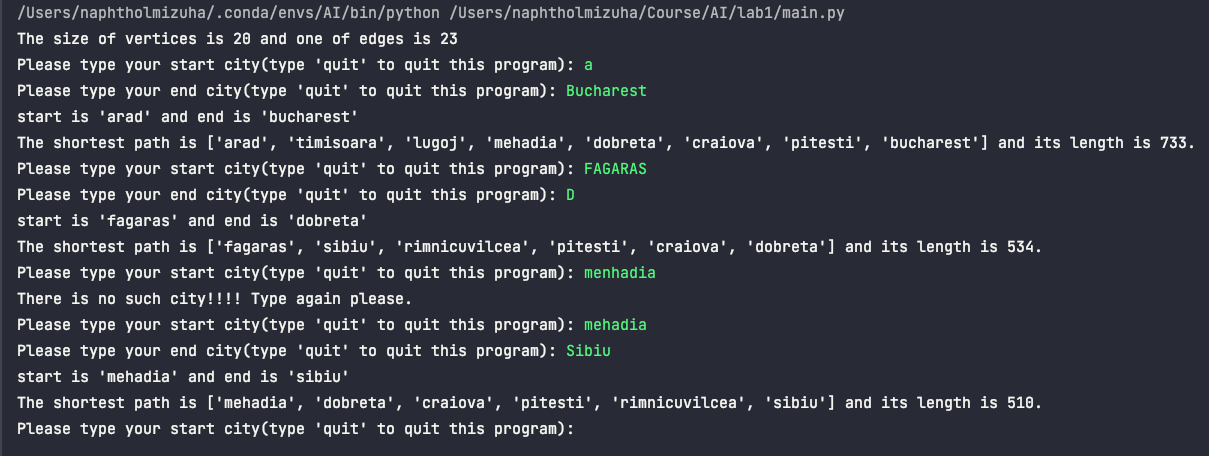
\includegraphics[scale=0.3]{res}
    \end{figure}
    \newpage
    而log.txt中的日志信息如下:
    \begin{figure}[htbp]\label{fig:figure2}
        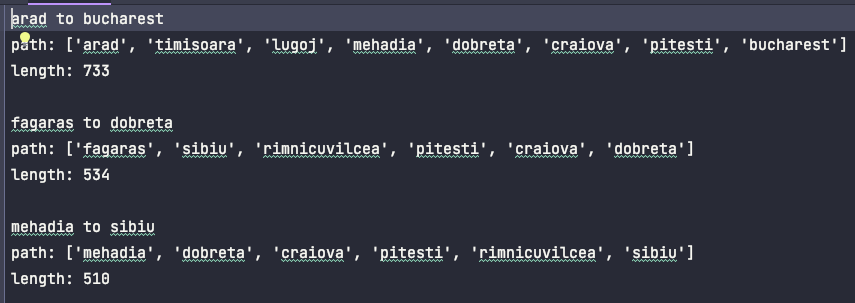
\includegraphics[scale=0.4]{log}
    \end{figure}

    不难看出,程序运行正确。主要体现在以下方面:
    \begin{enumerate}
        \item 输入首字母或城市全名均能正确识别。
        \item 实现了大小写无关。
        \item 成功得出了最短路径及其长度。
        \item 正确生成日志信息。
    \end{enumerate}

    \section{思考题}
    \subsection{字典的键}
    使用thinking.py脚本验证:
    \pythonfile{thinking.py}
    发现解释器在第6行报错,并提示list并不是一个可哈希的类型。将第6行注释后,再次运行得到如下结果:
    \begin{figure}[htbp]\label{fig:figure3}
        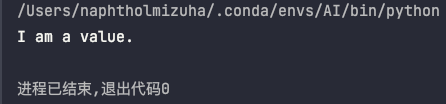
\includegraphics[scale=0.5]{value}
    \end{figure}
    根据观察可以得出:列表作为字典的键将会报错,而元组将可以正常使用运行。

    \subsection{可变/不可变}
    使用mutability.py脚本验证:
    \pythonfile{mutability.py}
    发现整数、浮点数、字符串、元组和布尔值变量在修改时会改变内存区域,即这些是不可变变量。而列表、集合和字典变量在修改后依然位于同一内存,即为可变变量。
\end{document}